% \documentclass[table]{beamer}
\documentclass[table,handout]{beamer}
\setbeameroption{show notes}
% \setbeameroption{hide notes}
% \setbeameroption{show only notes}
\usepackage{varwidth}

\newif\ifhide
\newif\ifpost
\newif\ifhideclicker

% \hidetrue
% \hideclickertrue
% \posttrue

\newcommand{\whiteout}[1]{\textcolor{white}{#1}}
% \newcommand{\whiteoutbox}[1]{\fcolorbox{white}{white}{\parbox{\dimexpr \linewidth-2\fboxsep-2\fboxrule}{\whiteout{#1}}}}
% \newcommand{\notebox}[1]{\fcolorbox{blue}{white}{\parbox{\dimexpr \linewidth-2\fboxsep-2\fboxrule}{#1}}}
\newcommand{\whiteoutbox}[1]{\fcolorbox{white}{white}{\parbox{\linewidth}{\whiteout{#1}}}}
\newcommand{\notebox}[1]{\fcolorbox{blue}{white}{\parbox{\linewidth}{#1}}}
\newcommand{\blankbox}[1]{\phantom{\varwidth{\linewidth}\whiteoutbox{#1}\endvarwidth}}
\newcommand{\blank}[1]{\phantom{\varwidth{\linewidth}#1\endvarwidth}}

\ifhide%
    \newcommand{\hmask}[1]{\blank{#1}}%
\else%
    \newcommand{\hmask}[1]{#1}%
\fi

\ifhide%
    \newcommand{\wout}[1]{\whiteout{#1}}%
\else%
    \newcommand{\wout}[1]{#1}%
\fi

\ifhide%
    \newcommand{\hignore}[1]{}%
\else%
    \newcommand{\hignore}[1]{#1}%
\fi

\ifpost%
    \newcommand{\nopost}[1]{}%
\else%
    \newcommand{\nopost}[1]{#1}%
\fi

\ifhideclicker%
    \newcommand{\clickerslide}[1]{\stepcounter{clickerQuestionCounter}%
        \begin{frame}[t]
            \textcolor{blue}{Q \arabic{clickerQuestionCounter}:}
        \end{frame}}
\else%
    \newcommand{\clickerslide}[1]{#1}%
\fi

\ifhide%
    \newcommand{\hidebox}[1]{\blank{#1}}%
\else%
    \newcommand{\hidebox}[1]{\notebox{#1}}%
\fi

\ifhide%
    \newcommand{\wbox}[1]{\whiteoutbox{#1}}%
\else%
    \newcommand{\wbox}[1]{\notebox{#1}}%
\fi

\ifhide%
    \newcommand{\nbox}[1]{\blankbox{#1}}%
\else%
    \newcommand{\nbox}[1]{\notebox{#1}}%
\fi

\ifhideclicker%
    \newcommand{\clickeranswer}[1]{#1}%
\else%
    \ifhide%
        \newcommand{\clickeranswer}[1]{#1}%
    \else%
        \newcommand{\clickeranswer}[1]{\textbf{\textcolor{blue}{#1}}}%
    \fi
\fi

\usepackage{beamerthemesplit}
% \usetheme{boxes}
\usetheme{Malmoe}
\usecolortheme{seahorse}
% \usecolortheme{seagull}
\usepackage{ifthen}
\usepackage{xspace}
\usepackage{multirow}
\usepackage{multicol}
\usepackage{booktabs}
\usepackage{xcolor}
\usepackage{wasysym}
\usepackage{comment}
\usepackage{hyperref}
\hypersetup{pdfborder={0 0 0}, colorlinks=true, urlcolor=blue, linkcolor=blue, citecolor=blue}
\usepackage{changepage}
\usepackage[compatibility=false]{caption}
\captionsetup[figure]{font=scriptsize, labelformat=empty, textformat=simple, justification=centering, skip=2pt}
\usepackage{tikz}
\usetikzlibrary{trees,calc,backgrounds}

\usepackage[bibstyle=joaks-slides,maxcitenames=3,mincitenames=1,backend=biber]{biblatex}

\newrobustcmd*{\shortfullcite}{\AtNextCite{\renewbibmacro{title}{}\renewbibmacro{in:}{}\renewbibmacro{number}{}}\fullcite}

\newrobustcmd*{\footlessfullcite}{\AtNextCite{\renewbibmacro{title}{}\renewbibmacro{in:}{}}\footfullcite}

% Make all footnotes smaller
% \renewcommand{\footnotesize}{\scriptsize}

\definecolor{myGray}{gray}{0.9}
\colorlet{rowred}{red!30!white}

\setbeamertemplate{blocks}[rounded][shadow=true]

\setbeamercolor{defaultcolor}{bg=structure!30!normal text.bg,fg=black}
\setbeamercolor{block body}{bg=structure!30!normal text.bg,fg=black}
\setbeamercolor{block title}{bg=structure!50!normal text.bg,fg=black}

\newenvironment<>{varblock}[2][\textwidth]{%
  \setlength{\textwidth}{#1}
  \begin{actionenv}#3%
    \def\insertblocktitle{#2}%
    \par%
    \usebeamertemplate{block begin}}
  {\par%
    \usebeamertemplate{block end}%
  \end{actionenv}}

\newenvironment{displaybox}[1][\textwidth]
{
    \centerline\bgroup\hfill
    \begin{beamerboxesrounded}[lower=defaultcolor,shadow=true,width=#1]{}
}
{
    \end{beamerboxesrounded}\hfill\egroup
}

\newenvironment{onlinebox}[1][4cm]
{
    \newbox\mybox
    \newdimen\myboxht
    \setbox\mybox\hbox\bgroup%
        \begin{beamerboxesrounded}[lower=defaultcolor,shadow=true,width=#1]{}
    \centering
}
{
    \end{beamerboxesrounded}\egroup
    \myboxht\ht\mybox
    \raisebox{-0.25\myboxht}{\usebox\mybox}\hspace{2pt}
}

\newenvironment{mydescription}{
    \begin{description}
        \setlength{\leftskip}{-1.5cm}}
    {\end{description}}

\newenvironment{myitemize}{
    \begin{itemize}
        \setlength{\leftskip}{-.3cm}}
    {\end{itemize}}

% footnote without a marker
\newcommand\barefootnote[1]{%
  \begingroup
  \renewcommand\thefootnote{}\footnote{#1}%
  \addtocounter{footnote}{-1}%
  \endgroup
}

% define formatting for footer
\newcommand{\myfootline}{%
    {\it
    \insertshorttitle
    \hspace*{\fill} 
    \insertshortauthor, \insertshortinstitute
    % \ifx\insertsubtitle\@empty\else, \insertshortsubtitle\fi
    \hspace*{\fill}
    \insertframenumber/\inserttotalframenumber}}

% set up footer
\setbeamertemplate{footline}{%
    \usebeamerfont{structure}
    \begin{beamercolorbox}[wd=\paperwidth,ht=2.25ex,dp=1ex]{frametitle}%
        % \Tiny\hspace*{4mm}\myfootline\hspace{4mm}
        \tiny\hspace*{4mm}\myfootline\hspace{4mm}
    \end{beamercolorbox}}

% remove navigation bar
\beamertemplatenavigationsymbolsempty

\makeatletter
    \newenvironment{noheadline}{
        \setbeamertemplate{headline}[default]
        \def\beamer@entrycode{\vspace*{-\headheight}}
    }{}
\makeatother

\newcounter{clickerQuestionCounter}
\ifhideclicker%
\newenvironment{clickerquestion}
{ \stepcounter{clickerQuestionCounter}
  \begin{enumerate}[Q \arabic{clickerQuestionCounter}:]\color{white} }
{ \end{enumerate} }
\else%
\newenvironment{clickerquestion}
{ \stepcounter{clickerQuestionCounter}
  \begin{enumerate}[Q \arabic{clickerQuestionCounter}:] }
{ \end{enumerate} }
\fi

\ifhideclicker%
\newenvironment{clickeroptions}
{ \begin{enumerate}[\begingroup\color{white} 1)\endgroup]\color{white} }
{ \end{enumerate} }
\else%
\newenvironment{clickeroptions}
{ \begin{enumerate}[\begingroup\color{red} 1)\endgroup] }
{ \end{enumerate} }
\fi


\tikzstyle{centered} = [align=center, text centered, font=\sffamily\bfseries]
\tikzstyle{skip} = [centered, inner sep=0pt, fill]
\tikzstyle{empty} = [centered, inner sep=0pt]
\tikzstyle{inode} = [centered, circle, minimum width=4pt, fill=black, inner sep=0pt]
\tikzstyle{tnode} = [centered, circle, inner sep=1pt]
\tikzset{
  % edge styles
  level distance=10mm,
  mate/.style={edge from parent/.style={draw,distance=3pt}},
  mleft/.style={grow=left, level distance=10mm, edge from parent path={(\tikzparentnode.west)--(\tikzchildnode.east)}},
  mright/.style={grow=right, level distance=10mm, edge from parent path={(\tikzparentnode.east)--(\tikzchildnode.west)}},
  % node styles
  male/.style={rectangle,minimum size=4mm,fill=gray!80},
  female/.style={circle,minimum size=4mm,fill=gray!80},
  amale/.style={male,fill=red},
  afemale/.style={female,fill=red},
}

\newcommand{\highlight}[1]{\textcolor{violet}{\textit{\textbf{#1}}}}
\newcommand{\super}[1]{\ensuremath{^{\textrm{\sffamily #1}}}}
\newcommand{\sub}[1]{\ensuremath{_{\textrm{\sffamily #1}}}}
\newcommand{\dC}{\ensuremath{^\circ{\textrm{C}}}}
\newcommand{\tb}{\hspace{2em}}
\providecommand{\e}[1]{\ensuremath{\times 10^{#1}}}
\newcommand{\myHangIndent}{\hangindent=5mm}

\newcommand{\spp}[1]{\textit{#1}}

\newcommand\mybullet{\leavevmode%
\usebeamertemplate{itemize item}\hspace{.5em}}

\makeatletter
\newcommand*{\rom}[1]{\expandafter\@slowromancap\romannumeral #1@}
\makeatother

\newcommand{\blankslide}{{\setbeamercolor{background canvas}{bg=black}
\setbeamercolor{whitetext}{fg=white}
\begin{frame}<handout:0>[plain]
\end{frame}}}

\newcommand{\whiteslide}{
\begin{frame}<handout:0>[plain]
\end{frame}}

\newcommand{\f}[1]{\ensuremath{F_{#1}}}
\newcommand{\x}[1]{X\ensuremath{^{#1}}}
\newcommand{\y}[1]{Y\ensuremath{^{#1}}}

% Population growth macros
\newcommand{\popsize}[1]{\ensuremath{N_{#1}}}
\newcommand{\popgrowthratediscrete}[1]{\ensuremath{\lambda_{#1}}}
\newcommand{\popgrowthrate}[1]{\ensuremath{r_{#1}}}
\newcommand{\ptime}{\ensuremath{t}\xspace}

\tikzset{hide on/.code={\only<#1>{\color{white}}}}
\tikzset{
    invisible/.style={opacity=0},
    visible on/.style={alt={#1{}{invisible}}},
    alt/.code args={<#1>#2#3}{%
        \alt<#1>{\pgfkeysalso{#2}}{\pgfkeysalso{#3}}
        % \pgfkeysalso doesn't change the path
    },
}

\bibliography{../bib/references}
\author[J.\ Oaks]{
    %Jamie R.\ Oaks\inst{1}
    Jamie R.\ Oaks
}
\institute[BIOL 180]{
    \inst{}%
        BIOL 180: Introductory Biology
}



\title[Behavioral ecology \& sexual selection]{Behavioral ecology \& sexual
    selection}
% \date{\today}
\date{May 12, 2015}


% \setbeamertemplate{section in toc}[sections numbered]
% \setbeamertemplate{subsection in toc}[subsections numbered]

\begin{document}

\begin{noheadline}
\maketitle
\end{noheadline}


\nopost{
\begin{noheadline}
\begin{frame}[c]
    \vspace{-6mm}
    \begin{center} 
        \includegraphics[height=1.2\textheight]{../images/seating-chart-2.pdf}
    \end{center}
\end{frame}
\end{noheadline}
}

\clickerslide{
\begin{noheadline}
\begin{frame}
    \begin{clickerquestion}
        \item Recent data suggest that limited interbreeding occurred between
            \textit{H.\ sapiens} and \textit{H.\ neanderthalensis}. Does this
            mean that they are actually the same species? 

        \begin{clickeroptions}
            \item Yes---they were not reproductively isolated so they were not
                evolutionary independent units in nature. 
            \item Yes---both \textit{H.\ sapiens} and Neanderthals had
                language, buried their dead, used tools, and had other aspects
                of advanced culture.
            \item \clickeranswer{No---with only a small amount of
                    interbreeding, unique differences (synapomorphies) between
                    the species will be maintained.}
            \item No---they've always been considered separate species.
        \end{clickeroptions}
    \end{clickerquestion}
\end{frame}
\end{noheadline}
}

\begin{noheadline}
\begin{frame}
\frametitle{Today's issues:}
\vspace{5mm}
% \tableofcontents[subsectionstyle=hide]
\tableofcontents
\end{frame}
\end{noheadline}

\section[What are ecology and behavioral ecology?]{What are ecology and
    behavioral ecology?}

\begin{noheadline}
\begin{frame}[t]
    \frametitle{What are ecology and behavioral ecology?}
    \begin{adjustwidth}{-2em}{-1.5em}

        \begin{itemize}
            \item<1-> \textbf{Ecology:} The study of how organisms interact
                with each other and their environment.

                \vspace{4mm}
            \item<2-> \textbf{Behavior:} The study of what organisms do, how they
                do it (in terms of genetic/neuronal/hormonal mechanisms),
                and why (in terms of fitness).

                \vspace{4mm}
            \item<3-> \textbf{Behavioral ecology:} The study of how organisms
                make decisions when they interact with each other and various
                aspects of their environment.
        \end{itemize}
    \end{adjustwidth}
\end{frame}
\end{noheadline}

\begin{frame}[t]
    \begin{adjustwidth}{-2em}{-1.5em}
        Questions in behavioral ecology:

        \begin{itemize}
            \item What should I eat?

                \vspace{4mm}
            \item Where should I live?

                \vspace{4mm}
            \item How should I communicate?

                \vspace{4mm}
            \item Who should I mate with?

                \vspace{4mm}
            \item When should I cooperate?
        \end{itemize}
    \end{adjustwidth}
\end{frame}

\section[What is sexual selection?]{What is sexual selection?}

\begin{noheadline}
\begin{frame}[t]
    \frametitle{What is sexual selection?}
    \begin{adjustwidth}{-2em}{-1.5em}
        \ldots background for addressing ``who should I mate with?''

        \uncover<2->{
        \vspace{3mm}
        Darwin wanted to explain why, in some species, males look different than
        females.
        }

        \begin{enumerate}
            \item<3-> There is heritable variation in appearance and/or
                courtship behavior.

                \vspace{5mm}
            \item<4-> Individuals experience differential success in obtaining
                mates---individuals with certain traits have more offspring.
        \end{enumerate}
    \end{adjustwidth}
\end{frame}
\end{noheadline}

\clickerslide{
\begin{frame}
    \begin{clickerquestion}
        \item What is the essence of evolution by sexual selection? 

        \begin{clickeroptions}
            \item Eggs are expensive; sperm are cheap. 
            \item Males fight; females choose. 
            \item \clickeranswer{Alleles that lead to increased success in
                    mating increase in frequency.}
            \item In most environments, sexually reproduced offspring have
                higher fitness than asexually reproduced offspring.
        \end{clickeroptions}
    \end{clickerquestion}
\end{frame}
}

\begin{frame}[t]
    \begin{adjustwidth}{-2em}{-1.5em}
        In many species, females invest MUCH more in offspring than males do.
        For example:

        \uncover<2->{
        \vspace{4mm}
        Female red deer average 145 kg.\, and are pregnant for 8 months over
        the winter. Calves average 15 kg at birth and nurse for two months;
        they weigh about 55 kg at weaning.
        }

        \begin{columns}[t]
        
        \column{0.59\linewidth}

        \uncover<3->{
        % \vspace{8mm}
        Males average 200 kg, they contribute \ldots
        }

        \uncover<4->{
        \vspace{8mm}
         = asymmetry in parental investment
        }

        \column{0.4\linewidth}

        \vspace{-7mm}
        \uncover<2->{
        \begin{figure}
        \begin{center}
        \includegraphics[width=\columnwidth]{../images/red-deer.jpg}
        \caption{\tiny
            \href{http://upload.wikimedia.org/wikipedia/commons/d/df/Red_deer.jpg}{CC
                BY-SA 3.0}}
        \end{center}
        \end{figure}
        }

        \end{columns}

    \end{adjustwidth}
\end{frame}

\clickerslide{
\begin{frame}
    \begin{clickerquestion}
        \item Which of the following statements is correct? 

        \begin{clickeroptions}
            \item In most species, males are larger than females. 
            \item \clickeranswer{In most species, female RS is limited by
                    access to the resources required to breed.}
            \item In most species, male RS is limited by the ability to produce
                large amounts of sperm. 
            \item In most species, female RS is limited by the ability to
                obtain mates. 
        \end{clickeroptions}
    \end{clickerquestion}
\end{frame}
}

\section[How does sexual selection act when males compete for mates?]{How does
    sexual selection act when males compete for mates?}

\begin{noheadline}
\begin{frame}[t]
    \frametitle{How does sexual selection act when males compete for mates?}
    \begin{adjustwidth}{-2em}{-1.5em}
        \vspace{-2mm}
        In red deer, intense male-male competition occurs.

        \begin{columns}[t]

        \column{0.44\linewidth}

        \begin{enumerate}
            \item Which sex has higher variation in RS?

                \nbox{\scriptsize Males---note that modes are about the same,
                    but that males have a much wider distribution (= greater
                    variance).}

            \item In which sex would alleles associated with increased mating
                success increase faster?

                \nbox{\scriptsize Males---successful alleles can be passed on
                    to 20 or more offspring}
        \end{enumerate}

        \column{0.55\linewidth}

        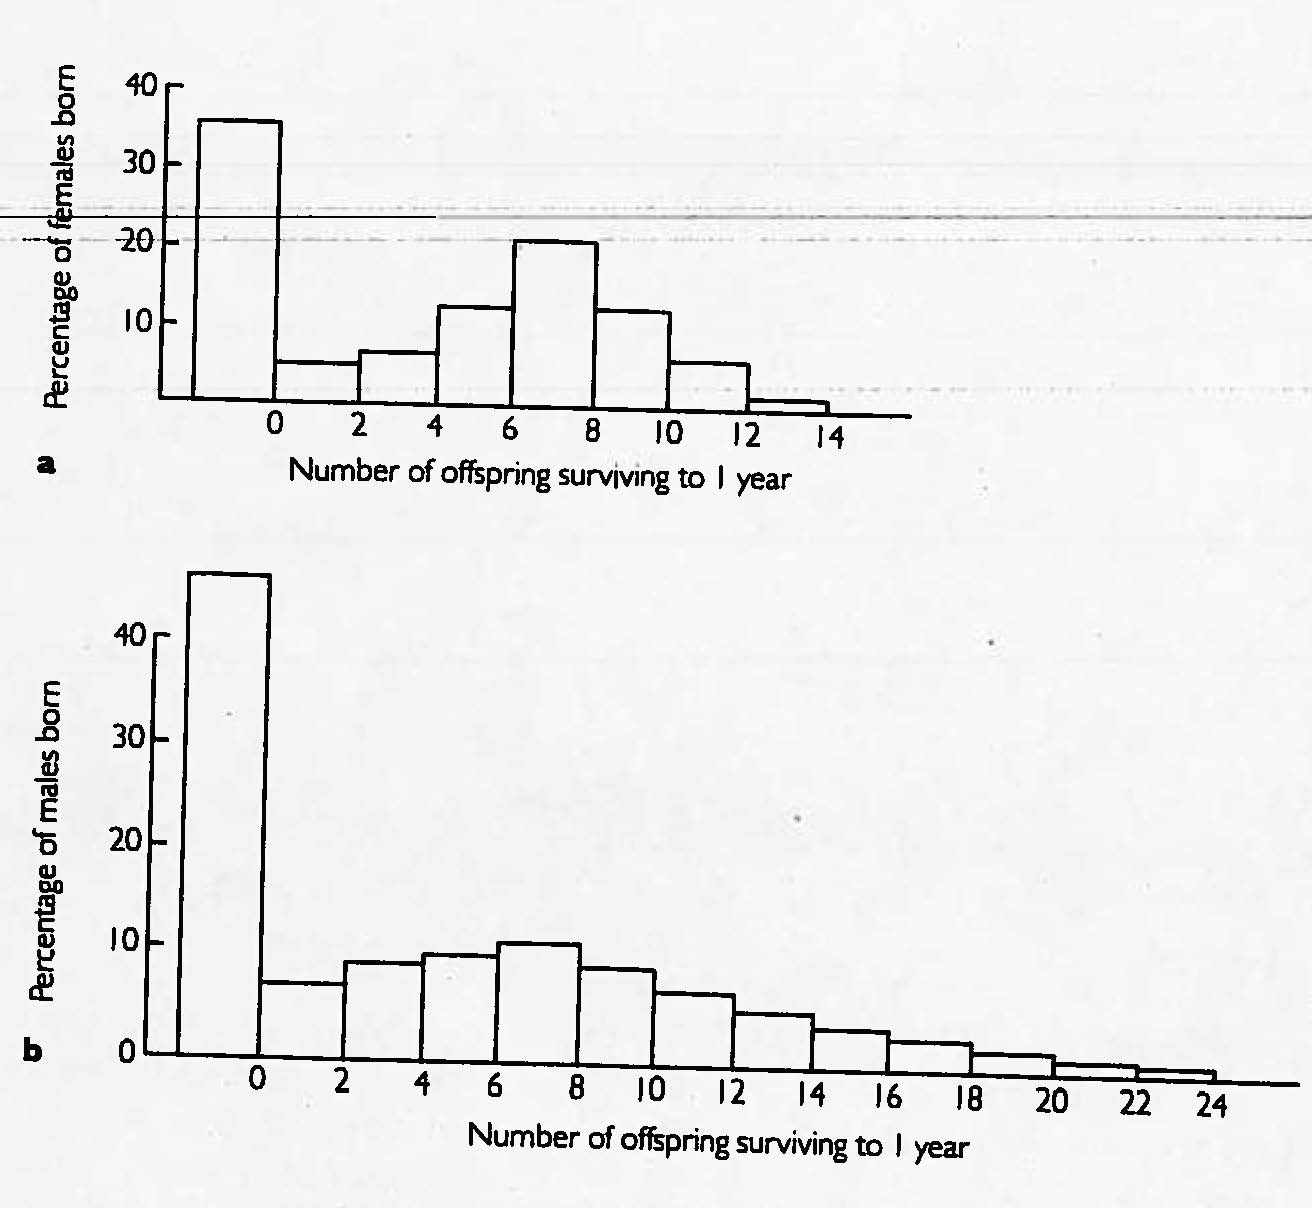
\includegraphics[width=\columnwidth]{deer-rs.jpg}

        \end{columns}
    \end{adjustwidth}
    \note[item]{Males establish harems. 1:1 sex ratio, but males exclude access
        to groups of 10 or so females. Other males have to fight to ``win'' a
        harem. Male-male combat (bigger one wins usually).}
\end{frame}
\end{noheadline}

\begin{frame}[t]
    \begin{adjustwidth}{-2em}{-1.5em}
        Observation: In some human cultures, men control access to jobs and
        other resources required to start a family, and marriages are arranged.
        As a result, females have little or no ability to choose their mates. 

        \vspace{5mm}
        Question: In these cultures, how might human behavioral ecology react
        to efforts to (1) increase the education level of women, or (2) help
        women start businesses through micro-lending or other programs? 

        \nbox{This is a discussion/opinion question \ldots but, answers should
            acknowledge that access to resources should increase the power that
            women have to choose their own mates.}

    \end{adjustwidth}
\end{frame}

\begin{frame}[t]
    \begin{adjustwidth}{-2em}{-1.5em}
        Observations:

        \begin{itemize}
            \item In the U.S., there is a strong correlation between
                level of educational attainment and lifetime income.
            
            \item Traditionally, men have been the family ``breadwinner.''

            \item Currently, 57\% of U.S.\ college students are female.
        \end{itemize}

        Question: In this culture, how might this new asymmetry in level of
        education affect society (= human behavioral ecology)?

        \nbox{This is a discussion/opinion question \ldots but, answers should
            acknowledge that traditional roles may reverse OR the correlation
            between education and income may break down.}

    \end{adjustwidth}
    \note[item]{Only 17\% of full professors are women.}
\end{frame}

\begin{frame}[t]
    \begin{adjustwidth}{-2em}{-1.5em}
        Observation: In China in 1996, there were 121 boys aged 1--4 for every
        100 girls aged 1--4. This cohort is almost of marriageable age.

        \begin{itemize}
            \item How likely is it that all men in this cohort will
                be able to marry and have a family?
            
                \nbox{Unlikely}

                \vspace{3mm}
            \item Will this situation make men happy or crabby?

                \nbox{\small Probably, many will be crabby}

                \vspace{3mm}
            \item How could this affect STDs?

                \nbox{\small Could increase sex trafficking??}

                \vspace{3mm}
            \item Boys are more esteemed than girls in traditional Chinese
                culture. Is this likely to change or remain the same?

                \nbox{\small ???}
        \end{itemize}

        \nbox{\scriptsize This is a discussion/opinion question \ldots but,
            answers should acknowledge that unbalanced sex ratios may have
            far-ranging social consequences.}

    \end{adjustwidth}
    \note[item]{Long-term trend! E.g., India: 33 million more men than women
        between ages 1--24}
\end{frame}

\section[How does sexual selection act when females choose mates?]{How does
    sexual selection act when females choose mates?}

\begin{frame}[t]
    \begin{adjustwidth}{-2em}{-1.5em}
        \vspace{-3mm}
        How does sexual selection act when females choose mates?

        \vspace{2mm}
        What do females choose?

        \begin{enumerate}
            \item ``Good alleles''
        \end{enumerate}

        \begin{columns}[t]

        \column{0.39\linewidth}

        Why is this male's plumage and display an ``honest'' advertisement of
        genetic quality?

        \nbox{\small If the male is sick or weakened by poor nutrition, his
            feathers would not be as bright, and he would not be able to
            display very well.}
        \nbox{\small NOTE: male birds of paradise do not help rear the young}

        \column{0.6\linewidth}
        
        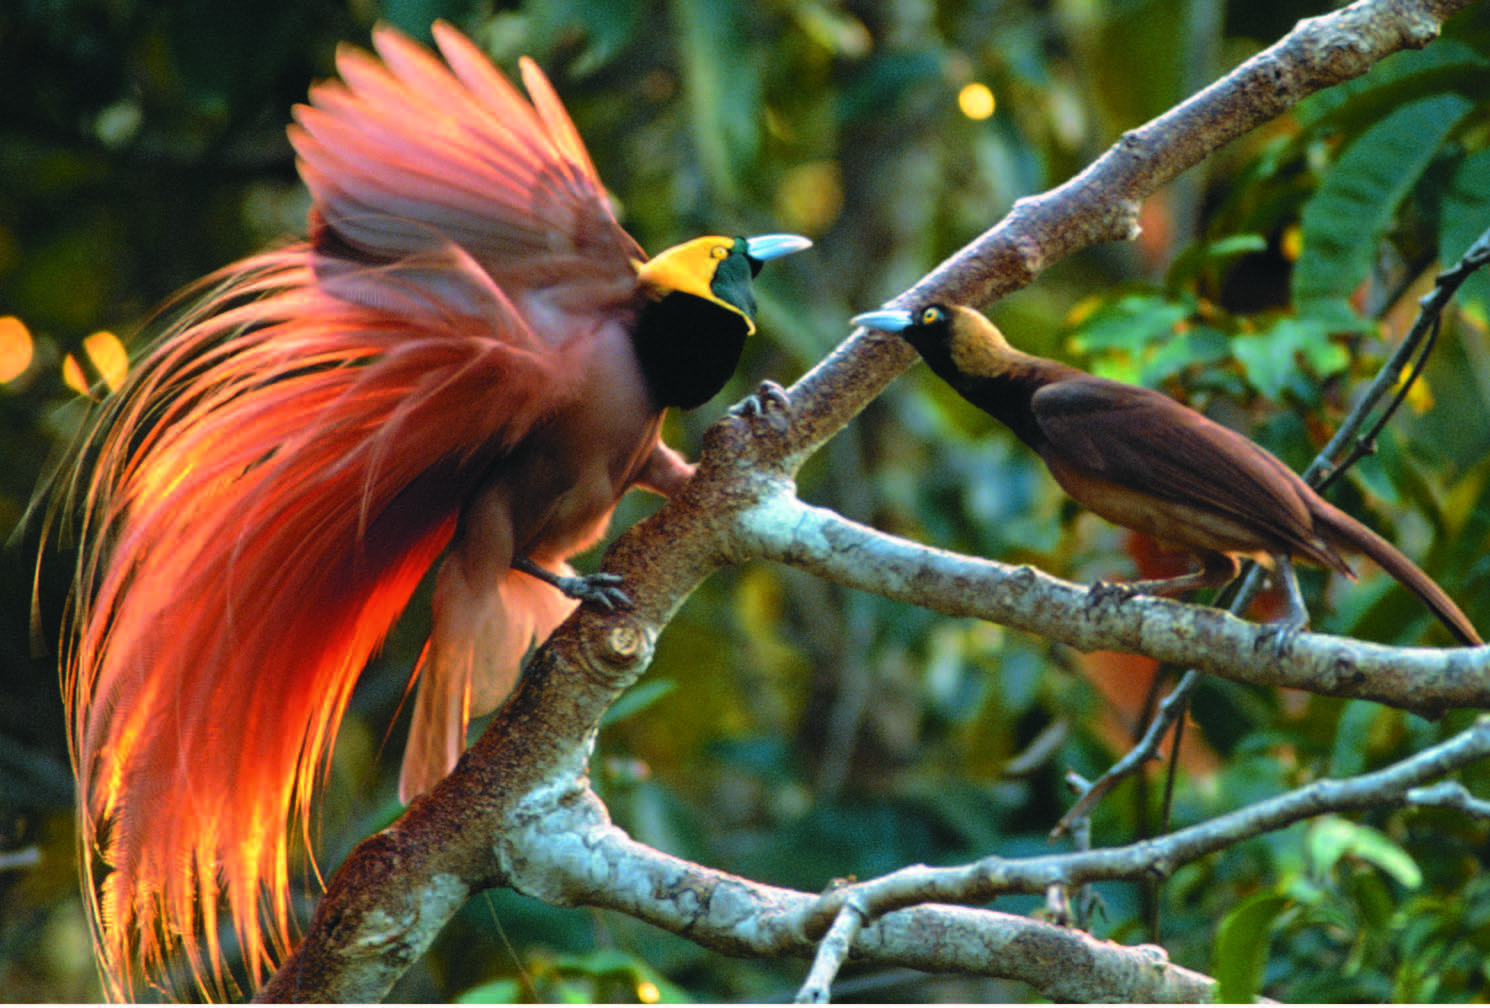
\includegraphics[width=\columnwidth]{bird-of-paradise.jpg}

        \end{columns}

    \end{adjustwidth}
\end{frame}

\begin{frame}[t]
    \begin{adjustwidth}{-2em}{-1.5em}
        \vspace{-3mm}
        How does sexual selection act when females choose mates?

        \vspace{2mm}
        What do females choose?

        \begin{enumerate}
            \addtocounter{enumi}{1}
            \item Resources required to produce offspring

            \uncover<2->{
                \vspace{1mm}
            E.g., Sexual selection in Australian redback spiders.
            } 
        \end{enumerate}

        \begin{columns}[t]

        \column{0.45\linewidth}

        \vspace{-5mm}
        \begin{itemize}
                \small
            \item<2-> During copulation, male redbacks insert palps (copulatory
                organ) into the female's sperm storage organ. (Longer
                copulation = more sperm transfered)

            \item<3-> Then, some males do a somersault, which places their
                abdomen in front of the female's mouthparts.

            \item<4-> In many cases, the female proceeds to eat the male.
        \end{itemize}

        \column{0.54\linewidth}
        
        \includegraphics<2->[width=\columnwidth]{spider.jpg}

        \end{columns}

    \end{adjustwidth}
\end{frame}

\begin{frame}[t]
    \begin{adjustwidth}{-2em}{-1.5em}
        Hypothesis: If male is eaten, the male is able to transfer more sperm
        (longer copulation). Also, the female gets resources to support eggs,
        and so is less likely to accept more matings.

        \vspace{4mm}
        Prediction: RS of cannibalized males is higher than RS of
        non-cannibalized males.

        \uncover<2->{
        \vspace{4mm}
        Test: Allow female redbacks to mate with two males.  Document whether
        or not she eats the 1\super{st} male, and whether or not she accepts
        the 2\super{nd} male.
        }   
    \end{adjustwidth}
\end{frame}

\begin{frame}[t]
    \begin{adjustwidth}{-2em}{-1.5em}
        Data:

        \vspace{4mm}
    \begin{table}%[htbp]
        \centering
        \begin{tabular}{ L{4.7cm} | C{3cm} | C{3cm} |}
            \multicolumn{1}{c}{} &
            \multicolumn{1}{c}{2\super{nd} male rejected} &
            \multicolumn{1}{c}{2\super{nd} male accepted} \\
            \cline{2-3}
            Females ate 1\super{st} male & 6 & 3 \\
            \cline{2-3}
            Females did not eat 1\super{st} male & 1 & 22 \\
            \cline{2-3}
        \end{tabular}
    \end{table}

    \begin{enumerate}
        \item<2-> What statistical test would you use to analyze these data?

            \nbox{Explanatory and response variables are both categorical:
                Goodness-of-fit test---e.g., Chi-square test}

            \vspace{5mm}
        \item<2->Test is significant (p-value $<$ 0.05). For males, is there a
            fitness benefit to being cannibalized?

            \nbox{Yes---the female is much more likely to use his sperm to
                fertilize all of her eggs.}
    \end{enumerate}

    \end{adjustwidth}
\end{frame}

\clickerslide{
\begin{frame}
    \begin{clickerquestion}
        \item For males, is there a fitness benefit to being cannibalized?
        \begin{clickeroptions}
            \item Yes---females are more likely to eat the second male.
            \item \clickeranswer{Yes---females are less likely to accept a
                    second mate, and so the male that was eaten is more likely
                    to fertilize all of her eggs.}
            \item No---the male died, and so his fitness is zero.
            \item No---the female is more likely to accept a second mate, and
                so the male that was eaten will fertilize only a portion of her
                eggs.
        \end{clickeroptions}
    \end{clickerquestion}
\end{frame}
}

\clickerslide{
\begin{frame}
    \begin{clickerquestion}
        \item Under what conditions is the mating system of the redback spider
            most likely to evolve?
        \begin{clickeroptions}
            \item Females are plentiful (males encounter them all the time).
            \item \clickeranswer{Females are rare (males encounter them
                    rarely).}
            \item Males are plentiful (females are approached by males all the
                time).
            \item Males are rare (females are approached by males rarely).
        \end{clickeroptions}
    \end{clickerquestion}
    \nbox{Only about 20\% of males ever encounter a female in their lifetime!
        If a male finds one, there is VERY little chance he will ever see
        another one. It will maximize his fitness to invest as much as possible
        into fertilizing and supporting as many of her eggs as he can.}
\end{frame}
}

\end{document}

\clickerslide{
\begin{frame}
    \begin{clickerquestion}
        \item 
        \begin{clickeroptions}
            \item 
            \item 
            \item 
            \item 
        \end{clickeroptions}
    \end{clickerquestion}
\end{frame}
}

\clickerpost{
{
\usebackgroundtemplate{\includegraphics[page=17,width=\paperwidth]{./24-Radiation-extinction.pdf}}
\begin{frame}[t,plain]
    \begin{adjustwidth}{-2em}{-1.5em}
        \cmask{Answer: 3}
    \end{adjustwidth}
\end{frame}
}
}

